\documentclass[a4paper,12pt]{letter}

\usepackage{tikz}
\usepackage{amsmath}
\usepackage{amssymb}
\usepackage{nopageno}
\usepackage{amsmath}
%\usepackage{enumitem}
% \usepackage{mathtools}
%\usepackage{eqnarray,amsmath}
\usepackage[a4paper, total={7.5in, 11.25in}]{geometry}
%\usepackage[margin=2.5cm]{geometry}
\usepackage[utf8]{inputenc}
\usepackage[T1]{fontenc}
\usepackage{lmodern}
%\usepackage{amsmath, amssymb}
\usepackage{setspace}
\setstretch{1.2}
\usepackage{pgfplots}
\pgfplotsset{compat=1.18}

\usetikzlibrary{calc,3d,decorations.pathmorphing,decorations.pathreplacing,decorations.markings,snakes,arrows.meta,calc,patterns}
\tikzset{snake it/.style={decorate, decoration=snake}}

\begin{document}

\begin{center}
 (KTXFI1EBNF) Physics I.  Homework No.~3\\ \smallskip
April~27,~2026
 \end{center}

\begin{enumerate}

\item Determine the acceleration of a proton $ m = 1.67 \cdot 10^{-27}\,\mathrm{kg} $ in an electric field of strength $ E = 100\,\mathrm{N/C}. $ How many times greater is this acceleration than the acceleration due to gravity?

% ----------------------------------------------------------------------------------------------------------------------------------------

\item An electron is launched with an initial velocity of $ v_0 = 2\cdot 10^6\,\mathrm{m/s} $ between two parallel charged plates, as shown in the figure. If the electric field strength between the plates is $ E = 2\,\mathrm{kN/C}, $ where does the electron hit the upper plate? Assume that the arrangement is in vacuum.

\begin{center}
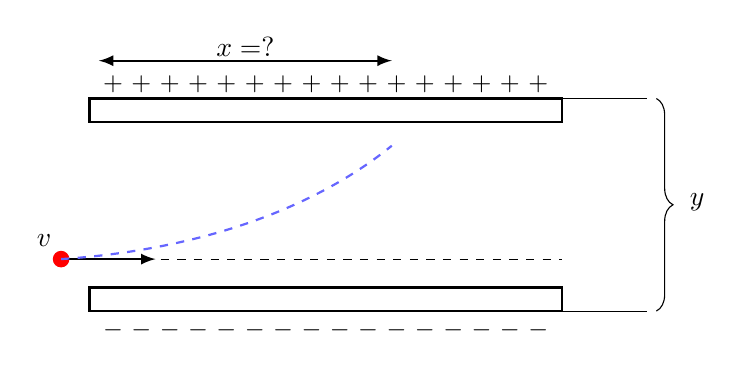
\begin{tikzpicture}[scale=1.2, >=latex]

% Plates
\draw[thick] (0,0) rectangle (5,0.25);
\draw[thick] (0,-2.0) rectangle (5,-1.75);

% Positive charges above upper plate
\foreach \x in {0.25,0.55,...,5.0}
{
    \node at (\x,0.4) {\small $+$};
}

% Negative charges below lower plate
\foreach \x in {0.25,0.55,...,5.0}
{
    \node at (\x,-2.2) {\small $-$};
}

% Electron
\fill[red] (-0.3,-1.45) circle (2.5pt);

% Initial velocity
\draw[->, thick] (-0.25,-1.45) -- (0.7,-1.45);
\node[left] at (-0.3,-1.25) {$v$};

% Dashed horizontal reference line
\draw[dashed] (-0.3,-1.45) -- (5.0,-1.45);

% Curved trajectory
\draw[dashed, thick, blue!60]
    (-0.3,-1.45) .. controls (1.2,-1.35) and (2.4,-0.9) .. (3.2,-0.25);

% x distance arrow
\draw[<->, thick] (0.1,0.65) -- (3.2,0.65);
\node at (1.65,0.8) {$x=?$};

% Vertical bracket for y
\draw[,thin] (5.6,0.25) -- (5.9,0.25);
\draw[thin] (5.6,-2.0) -- (5.9,-2.0);
\draw[decorate, decoration={brace, amplitude=6pt,mirror}]
    (6.0,-2.0) -- (6.0,0.25);
\node[right] at (6.25,-0.85) {$y$};

% Outer light guide lines
\draw[thin] (5.0,0.25) -- (5.6,0.25);
\draw[thin] (5.0,-2.0) -- (5.6,-2.0);

\end{tikzpicture}
%\caption{Electron motion between two parallel charged plates.}
\end{center}

% ----------------------------------------------------------------------------------------------------------------------------------------

\item An electron enters the region between the plate pair shown in the figure halfway between the plates. The length of the plates is $ l = 10\,\mathrm{cm}, $ their separation is $ d = 1\,\mathrm{cm}, $ and the voltage between them is $ U = 200\,\mathrm{V}. $ What must the initial velocity of the electron be if we want it to just barely leave the region between the plates?

\begin{center}
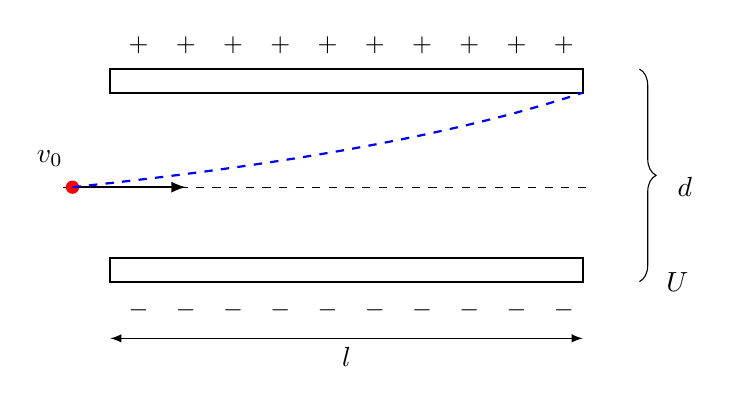
\begin{tikzpicture}[scale=1.2, >=latex]

% Parameters (for clarity)
\def\L{5}    % plate length
\def\d{2}    % plate distance

% Plates
\draw[thick] (0,0) rectangle (\L,0.25);
\draw[thick] (0,-\d) rectangle (\L,-\d+0.25);

% Positive charges (upper plate)
\foreach \x in {0.3,0.8,...,4.8}
{
    \node at (\x,+0.5) {\small $+$};
}

% Negative charges (lower plate)
\foreach \x in {0.3,0.8,...,4.8}
{
    \node at (\x,-2.3) {\small $-$};
}

% Midline (entry level)
\draw[dashed] (-0.5,-\d/2) -- (\L+0.1,-\d/2);

% Electron entry point
\fill[red] (-0.4,-\d/2) circle (2pt);

% Initial velocity
\draw[->, thick] (-0.4,-\d/2) -- (0.8,-\d/2);
\node[left] at (-0.4,-\d/2+0.3) {$v_0$};

% Curved trajectory (just touching upper plate at exit)
\draw[thick, dashed, blue]
    (-0.4,-\d/2) .. controls (1.5,-\d/2+0.2) and (3.5,-0.5) .. (\L,0.0);

% Length l
\draw[<->] (0,-\d-0.6) -- (\L,-\d-0.6);
\node at (\L/2,-\d-0.8) {$l$};

% Distance d (brace)
\draw[decorate, decoration={brace, amplitude=6pt, mirror}]
    (\L+0.6,-\d) -- (\L+0.6,0.25);
\node[right] at (\L+0.9,-\d/2) {$d$};

% Voltage label
\node at (\L+1.0,-\d/2-1.0) {$U$};

\end{tikzpicture}
%\caption{Electron motion between parallel plates (Problem 3).}
\end{center}

\end{enumerate}

% ----------------------------------------------------------------------------------------------------------------------------------------

\bigskip

\rightline{Dr.~Gabor~FACSKO}
\rightline{\textit{facsko.gabor@uni-obuda.hu}}

\vfill

\end{document}
